\documentclass{article}

\usepackage[utf8]{inputenc}
\usepackage[italian]{babel}
\usepackage{wrapfig}
\usepackage{hyperref}
\usepackage{listings}
\usepackage{amsfonts} 
\usepackage[table]{xcolor}
\usepackage{makecell}
\usepackage[table]{xcolor}
\usepackage{enumerate}
\usepackage[shortlabels]{enumitem}
\renewcommand{\arraystretch}{1.4}
\usepackage{array, cellspace}
\setlength{\cellspacetoplimit}{4pt}
\setlength{\cellspacebottomlimit}{4pt}
\usepackage{graphicx}
\usepackage{svg}
\usepackage{amsmath}
\usepackage[export]{adjustbox} 
\usepackage{float}
\usepackage{tabularx} % Da inserire nel preambolo se non già presente
\usepackage[utf8]{inputenc}
\usepackage[T1]{fontenc}
\usepackage{geometry}
\usepackage{array}
\usepackage{amsmath}
\usepackage{graphicx}
\usepackage{longtable}
\usepackage{listings}
\usepackage{xcolor}


\geometry{margin=2.5cm}
\setlength{\parskip}{0.5em}
\setlength{\parindent}{0pt}
\usepackage{
        geometry,
	plain,
	setspace, 
	titlesec,
}

\geometry{
	paperheight = 29.7cm,
	paperwidth = 21cm,
        left = 2.5cm,
        right = 2.5cm,
	top = 2cm,
	bottom = 2cm
}
\lstdefinestyle{ocl}{
  backgroundcolor=\color{gray!10},
  basicstyle=\ttfamily\small,
  breaklines=true,
  frame=single,
  rulecolor=\color{black},
  captionpos=b,
  tabsize=2,
  language=OCL
}
\singlespacing

\usepackage{blindtext}
\usepackage{nameref}

\newcounter{mylabelcounter}

\makeatletter
\newcommand{\labelText}[2]{%
#1\refstepcounter{mylabelcounter}%
\immediate\write\@auxout{%
  \string\newlabel{#2}{{1}{\thepage}{{\unexpanded{#1}}}{mylabelcounter.\number\value{mylabelcounter}}{}}%
}%
}
\makeatother

\begin{document}



\pagestyle{plain}
\thispagestyle{empty}

\graphicspath{{assets/figures/}}

\begin{center}
        \vspace*{2cm}
        \huge\textsc{Progetto di Ingegneria del Software\\}
	\begin{figure}[h!]
		\centerline{
\includegraphics[width=1\textwidth]{Img/logo_unitn.eps}}
	\end{figure}

	\LARGE{Dipartimento di Ingegneria e Scienza dell’Informazione}

	\vspace{1 cm}

	\Large{
		Corso di Laurea:\\
		Ingegneria Informatica, delle Comunicazioni ed Elettronica
	}

	\vspace{1 cm}
	
	\Huge\textsc{EcoTrack\\}
	\vspace{1cm}
	\Large{Gruppo 1}
    
        \vspace{0.88cm}
        \begin{tabular}{ccc}
        Giulio Gualtiero & Jago Revrenna & Tommaso Onori \\
        234656 & 235081 & 234893 \\
        \end{tabular}

	\vspace{3cm}

	\Large{Anno Accademico 2024/2025}
\end{center}
\tableofcontents
\section{Diagramma Componenti}

\subsection{Diagramma dei Componenti}
\begin{figure}[H]
    \centering
    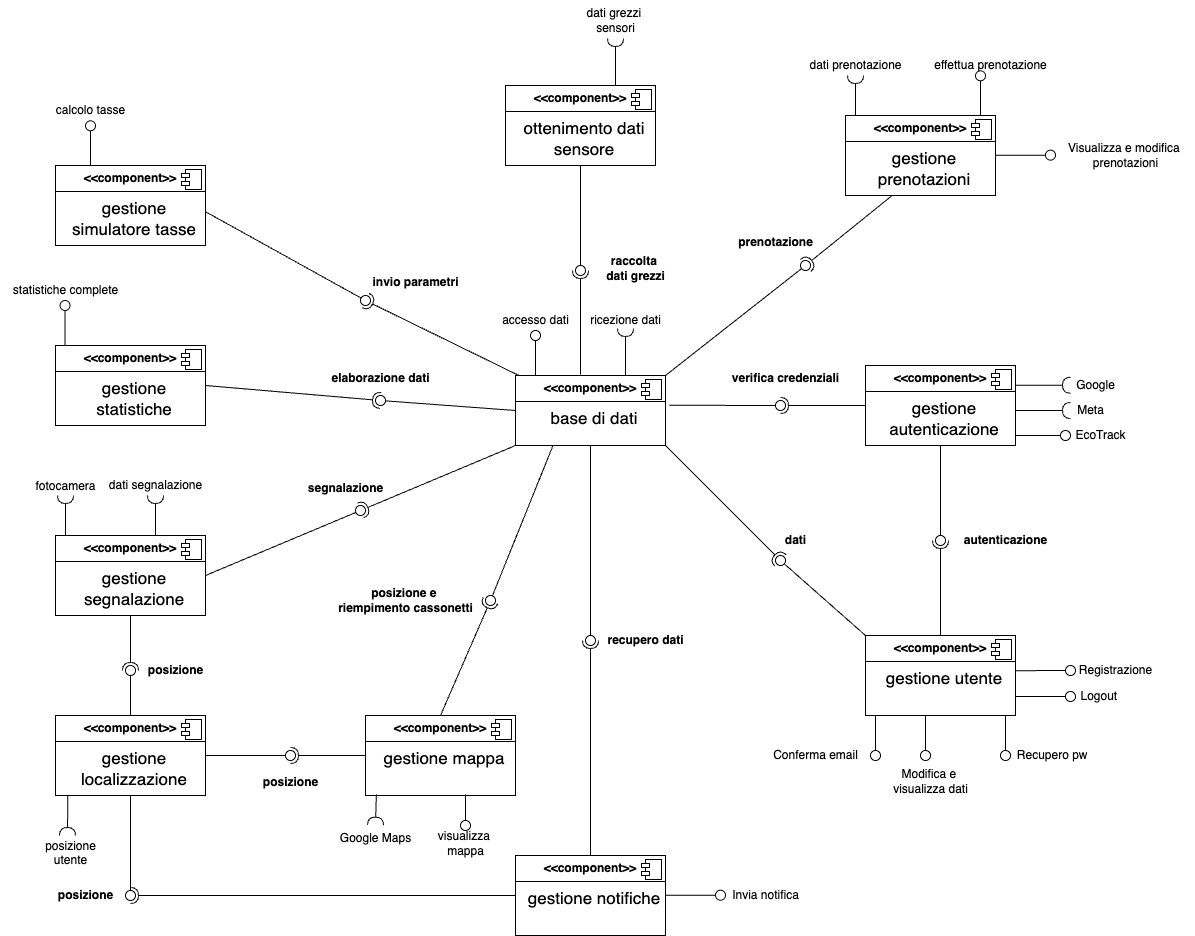
\includegraphics[width=1\linewidth]{D2-G1//Img/Component Diagram.png}
    \caption{Diagramma dei componenti}
    \label{fig:enter-label}
\end{figure}

\subsection{Descrizione dei Componenti}

\subsubsection{Gestione Autenticazione}  
Il componente gestisce l'autenticazione dell'utente, la quale può essere effettuata in diversi modi.

\begin{table}[H]
    \centering
    \begin{tabular}{|c|c|p{9cm}|}
        \hline
        \textbf{Tipologia} & \textbf{Nome} & \textbf{Descrizione} \\
        \hline
        Richiesta & Google & Il componente utilizza un’interfaccia fornita da Google per autenticarsi tramite un token (SSO) \\
        \hline
        Richiesta & Meta & Il componente utilizza un’interfaccia fornita da Meta per autenticarsi tramite un token (SSO) \\
        \hline
        Fornita & EcoTrack & Il componente fornisce un'interfaccia per autenticarsi mediante gli account locali \\
        \hline
        Fornita & Autenticazione & Il componente fornisce un'interfaccia per autenticarsi \\
        \hline
        Richiesta & Verifica credenziali & Il componente richiede che le credenziali vengano verificate \\
        \hline
    \end{tabular}
    \caption{Componenti coinvolti nella gestione dell'autenticazione}
    \label{tab:gestione_autenticazione}
\end{table}

\subsubsection{Gestione Localizzazione}  
Questo componente gestisce le interazioni con il sistema di localizzazione (GPS).

\begin{table}[H]
    \centering
    \begin{tabular}{|c|c|p{9cm}|}
        \hline
        \textbf{Tipologia} & \textbf{Nome} & \textbf{Descrizione} \\
        \hline
        Fornita & Posizione & Il componente fornisce (in coordinate) la posizione attuale dell'utente \\
        \hline
        Richiesta & Posizione utente & Il componente richiede la posizione attuale dell'utente \\
        \hline
    \end{tabular}
    \caption{Componenti coinvolti nella gestione della localizzazione}
    \label{tab:gestione_localizzazione}
\end{table}

\subsubsection{Base di Dati}  
Questo componente gestisce tutti i dati coinvolti nel funzionamento dell'applicazione e permette agli altri componenti di relazionarsi.

\begin{table}[H]
    \centering
    \begin{tabular}{|c|c|p{9cm}|}
        \hline
        \textbf{Tipologia} & \textbf{Nome} & \textbf{Descrizione} \\
        \hline
        Fornito & Verifica credenziali & Il componente effettua la verifica delle credenziali utilizzate \\
        \hline
        Fornito & Prenotazione & Il componente verifica gli orari disponibili e salva una prenotazione \\
        \hline
        Richiesto & Raccolta dati grezzi & Il componente raccoglie i dati grezzi direttamente dai sensori \\
        \hline
        Richiesto & Invio parametri & Il componente salva i parametri relativi al simulatore tasse \\
        \hline
        Fornito & Elaborazione dati & Il componente fornisce i dati grezzi, che devono essere elaborati. In seguito, i dati elaborati verranno inviati al componente in questione. \\
        \hline
        Richiesto & Segnalazione & Il componente salva un'eventuale segnalazione e mostra le segnalazioni già salvate \\
        \hline
        Fornito & Posizione e riempimento cassonetti & Il componente fornisce la posizione (coordinate) e il livello di riempimento dei cassonetti \\
        \hline
        Fornito & Recupero dati & Il componente fornisce i dati che potrebbero far scaturire una notifica \\
        \hline
        Richiesto & Dati & Il componente richiede e mostra i dati relativi ai vari utenti \\
        \hline
    \end{tabular}
    \caption{Componenti coinvolti nella gestione della base di dati}
    \label{tab:base_dati}
\end{table}

\section{Diagramma e Descrizione delle Classi}

\subsection{Diagramma delle Classi}
\begin{figure}[H]
    \centering
    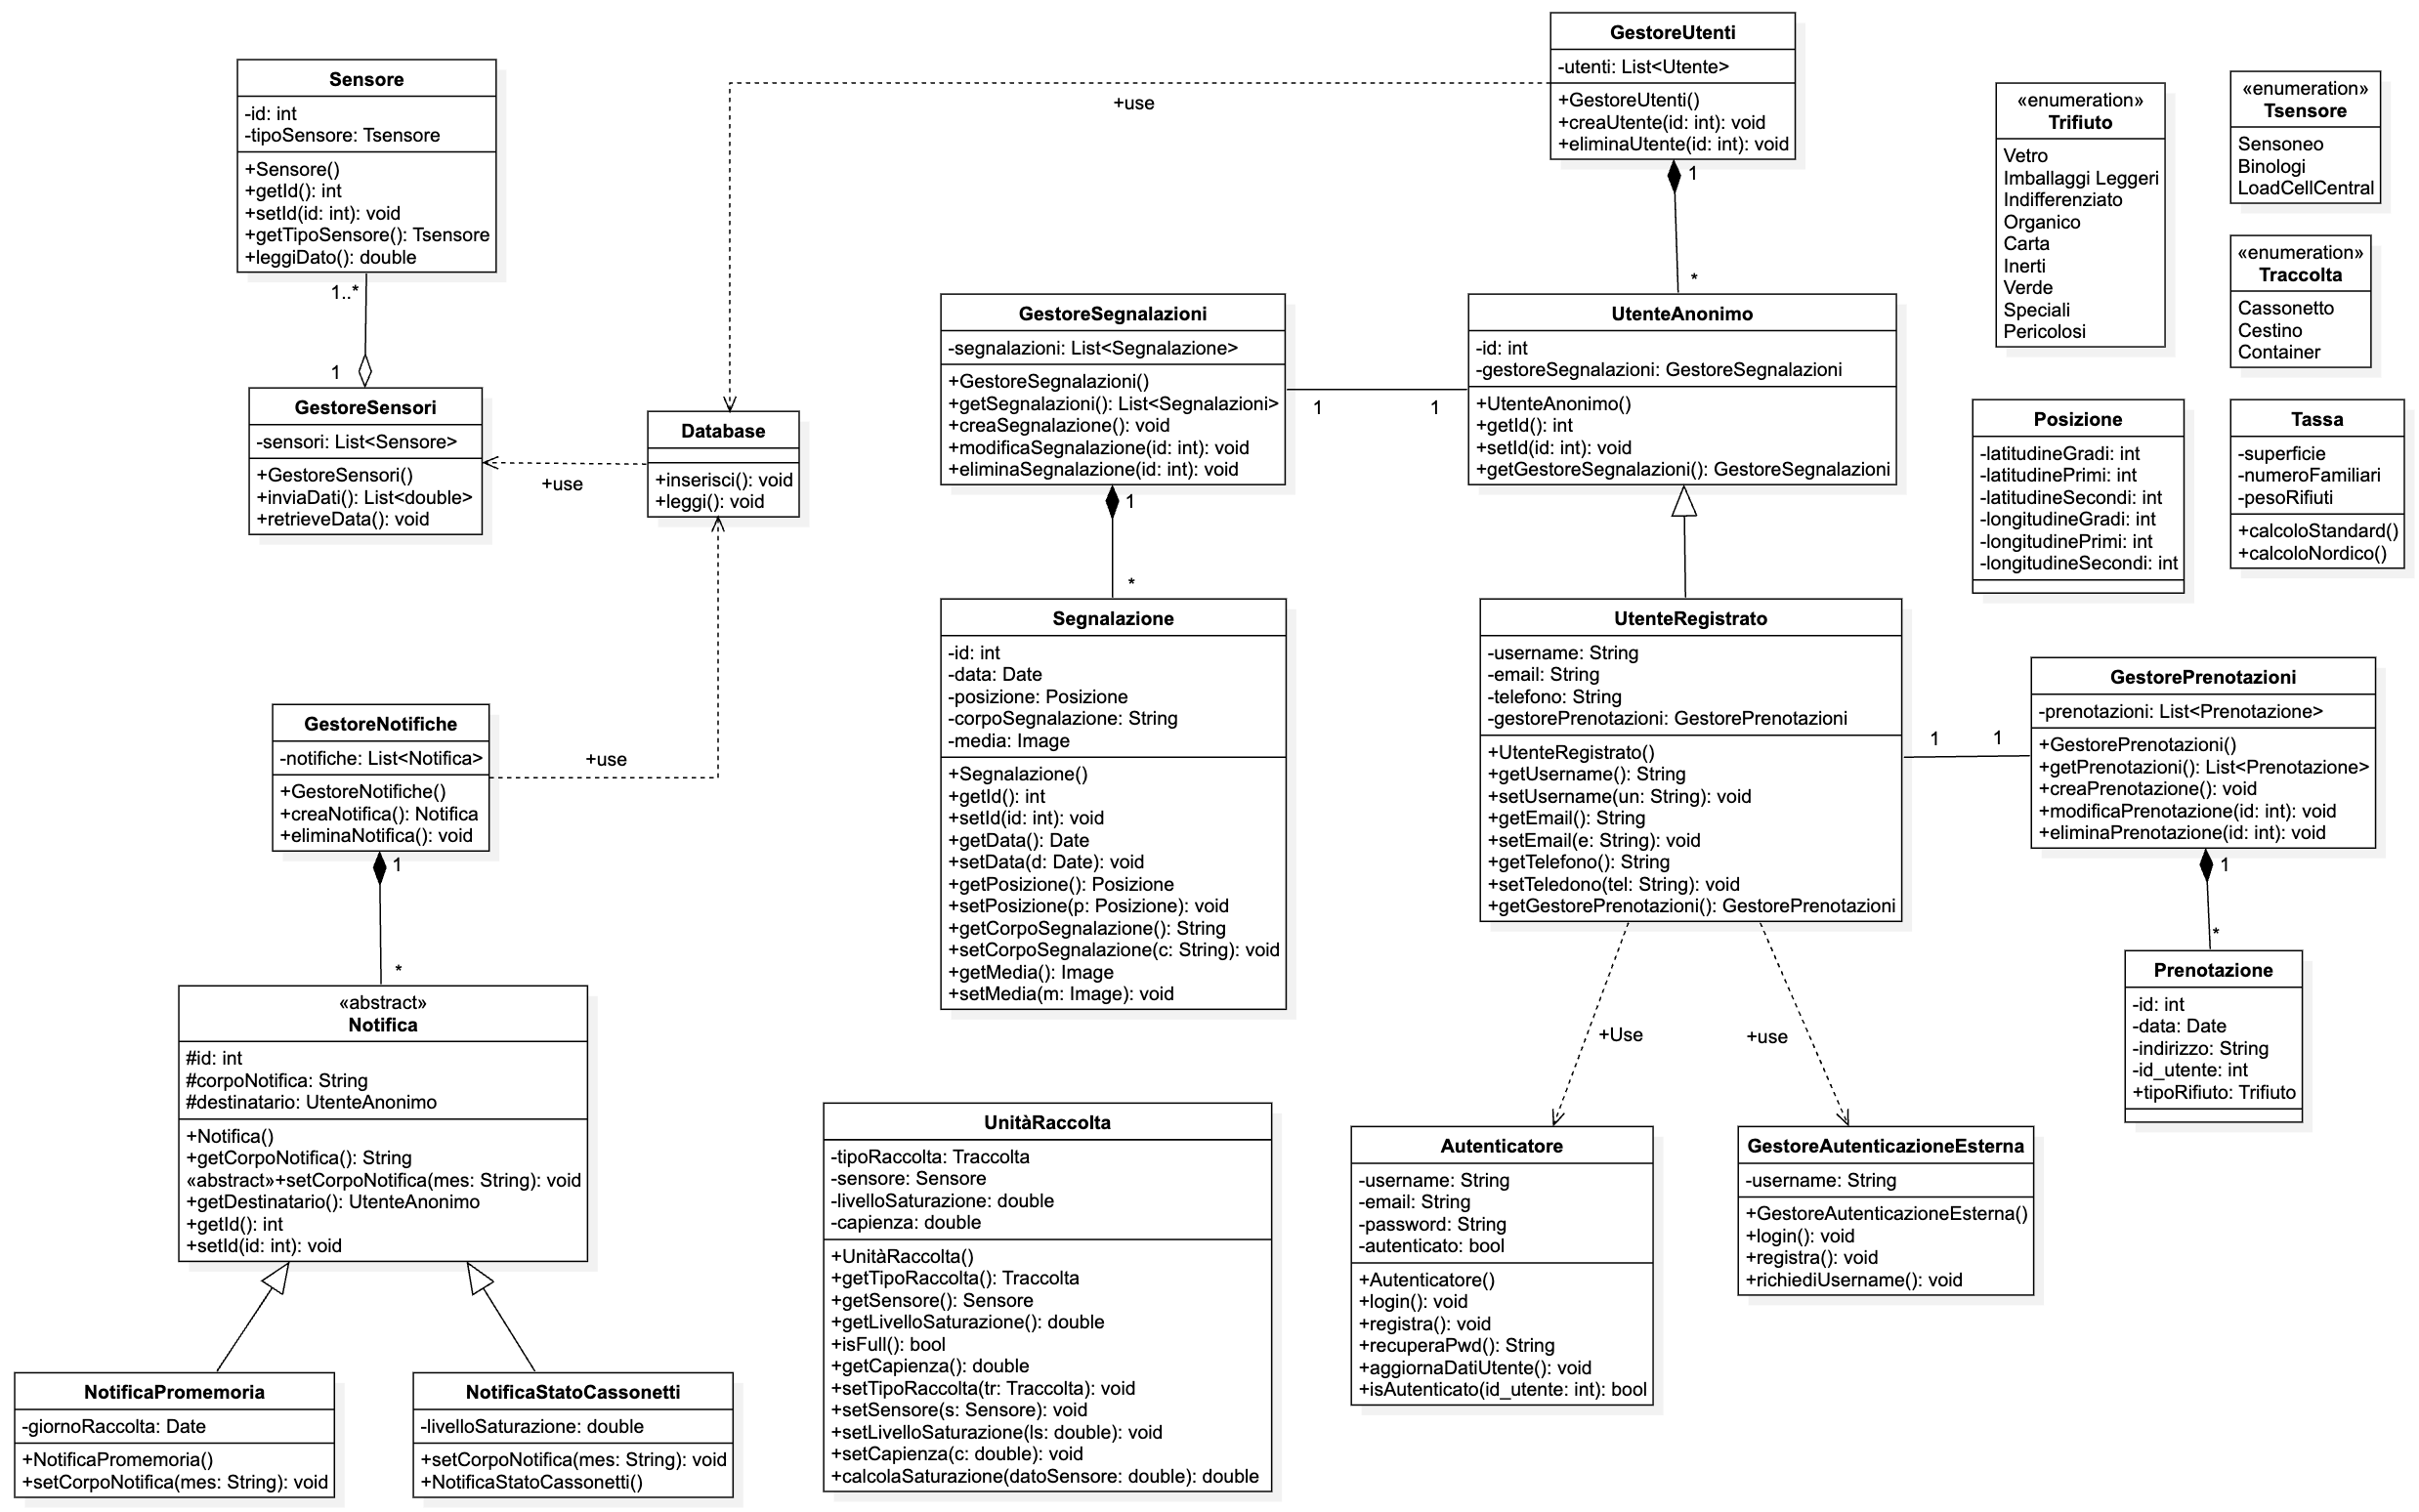
\includegraphics[width=1.05\linewidth]{D2-G1//Img/ClassDiagram.png}
    \caption{Diagramma delle Classi}
    \label{fig:enter-label}
\end{figure}

\subsection{Descrizione delle Classi}

\subsubsection{UtenteAnonimo}

La classe \textbf{UtenteAnonimo} rappresenta un utente non autenticato, che può comunque interagire con il sistema effettuando segnalazioni riguardanti problematiche o situazioni relative alla gestione dei rifiuti. Questa classe è pensata per garantire accesso a funzionalità base anche senza richiedere dati personali, mantenendo però una certa tracciabilità tramite un identificativo numerico.

\begin{table}[H]
\centering
\begin{tabularx}{\textwidth}{|l|X|}
\hline
\textbf{Metodo} & \textbf{Descrizione} \\
\hline
\texttt{UtenteAnonimo()} & Costruttore della classe, inizializza un nuovo utente anonimo con un gestore dedicato alle segnalazioni. \\
\hline
\texttt{getId()} & Restituisce l’identificativo numerico associato all’utente anonimo. \\
\hline
\texttt{setId(int id)} & Permette di impostare o aggiornare l’identificativo dell’utente. \\
\hline
\texttt{getGestoreSegnalazioni()} & Restituisce il riferimento all’oggetto incaricato di gestire le segnalazioni dell’utente. \\
\hline
\end{tabularx}
\caption{Metodi della classe \texttt{UtenteAnonimo}}
\end{table}

\subsubsection{UtenteRegistrato}

La classe \textbf{UtenteRegistrato} estende le funzionalità dell’utente anonimo offrendo servizi avanzati, tra cui la possibilità di gestire le prenotazioni per il ritiro dei rifiuti. L’utente fornisce informazioni personali al momento della registrazione e ha accesso a funzionalità aggiuntive.

\begin{table}[H]
\centering
\begin{tabularx}{\textwidth}{|l|X|}
\hline
\textbf{Metodo} & \textbf{Descrizione} \\
\hline
\texttt{UtenteRegistrato()} & Costruttore della classe. Inizializza un utente registrato e associa un gestore delle prenotazioni. \\
\hline
\texttt{getUsername()} & Restituisce il nome utente con cui l’utente è registrato nel sistema. \\
\hline
\texttt{setUsername(String un)} & Aggiorna lo username dell’utente. \\
\hline
\texttt{getEmail()} & Restituisce l’email associata all’account dell’utente. \\
\hline
\texttt{setEmail(String e)} & Permette di modificare l’indirizzo email. \\
\hline
\texttt{getTelefono()} & Restituisce il numero di telefono dell’utente. \\
\hline
\texttt{setTelefono(String tel)} & Aggiorna il numero di telefono. \\
\hline
\texttt{getGestorePrenotazioni()} & Restituisce l’oggetto incaricato della gestione delle prenotazioni per il ritiro dei rifiuti. \\
\hline
\end{tabularx}
\caption{Metodi della classe \texttt{UtenteRegistrato}}
\end{table}

\subsubsection{Autenticatore}

La classe \textbf{Autenticatore} si occupa della gestione dell’accesso al sistema da parte degli utenti. Fornisce metodi per l’autenticazione tramite credenziali, per la registrazione di nuovi account, per il recupero della password e per la verifica dello stato di autenticazione. Gestisce inoltre l’aggiornamento delle informazioni utente.

\begin{table}[H]
\centering
\begin{tabularx}{\textwidth}{|l|X|}
\hline
\textbf{Metodo} & \textbf{Descrizione} \\
\hline
\texttt{Autenticatore()} & Costruttore della classe. Inizializza un nuovo oggetto autenticatore. \\
\hline
\texttt{login()} & Verifica le credenziali fornite e autentica l’utente se valide. \\
\hline
\texttt{registra()} & Consente la registrazione di un nuovo utente nel sistema. \\
\hline
\texttt{recuperaPwd()} & Avvia la procedura di recupero password restituendo un link o codice temporaneo. \\
\hline
\texttt{aggiornaDatiUtente()} & Permette di aggiornare le informazioni personali dell’utente registrato. \\
\hline
\texttt{isAutenticato(int id\_utente)} & Verifica se l’utente con l’ID specificato ha completato l’autenticazione. \\
\hline
\end{tabularx}
\caption{Metodi della classe \texttt{Autenticatore}}
\end{table}

\subsubsection{GestoreAutenticazioneEsterna}

La classe \textbf{GestoreAutenticazioneEsterna} gestisce l’autenticazione attraverso provider esterni, come ad esempio Google o Facebook. Permette all’utente di accedere al sistema senza dover creare un account locale, semplificando il processo di login e registrazione. 

\begin{table}[H]
\centering
\begin{tabularx}{\textwidth}{|l|X|}
\hline
\textbf{Metodo} & \textbf{Descrizione} \\
\hline
\texttt{GestoreAutenticazioneEsterna()} & Costruttore della classe. Inizializza il gestore per l’interazione con provider esterni. \\
\hline
\texttt{login()} & legge le credenziali immesse dall’utente e chiama l’API del provider
esterno. In caso di successo aggiorna i valori degli attributi della classe
Utente (username e ID). \\
\hline
\texttt{registra()} & legge le credenziali immesse dall’utente e chiama l’API del provider
esterno. In caso di successo salva del Database i dati relativi all’utente. \\
\hline
\texttt{richiediUsername()} & richiede l’immissione di uno username in fase di registrazione tramite
provider esterno e lo salva nell’attributo username. \\
\hline
\end{tabularx}
\caption{Metodi della classe \texttt{GestoreAutenticazioneEsterna}}
\end{table}

\subsubsection{GestoreUtenti}

La classe \textbf{GestoreUtenti} rappresenta il componente incaricato della gestione centralizzata di tutti gli utenti della piattaforma, siano essi anonimi o registrati. Il gestore mantiene una collezione interna di utenti e fornisce operazioni per la loro creazione e rimozione. Questa classe garantisce coerenza e tracciabilità degli utenti attivi nel sistema, relazionandosi con il database così da poterla mantenere aggiornata.

\begin{table}[H]
\centering
\begin{tabularx}{\textwidth}{|l|X|}
\hline
\textbf{Metodo} & \textbf{Descrizione} \\
\hline
\texttt{GestoreUtenti()} & Costruttore della classe. Inizializza la struttura dati per contenere l’insieme degli utenti gestiti. \\
\hline
\texttt{creaUtente(int id)} & Aggiunge un nuovo utente al sistema, utilizzando l’identificativo fornito. \\
\hline
\texttt{eliminaUtente(int id)} & Rimuove l’utente corrispondente all’identificativo specificato, liberando eventuali risorse. \\
\hline
\end{tabularx}
\caption{Metodi della classe \texttt{GestoreUtenti}}
\end{table}

\subsubsection{GestoreSegnalazioni}

La classe \textbf{GestoreSegnalazioni} è responsabile della gestione delle segnalazioni inviate dagli utenti. Ogni istanza di questa classe gestisce un insieme di segnalazioni, offrendo funzionalità di visualizzazione, creazione, modifica e cancellazione (CRUD). È pensata per essere utilizzata da un ciascun utente, in modo da mantenere separate le segnalazioni.

\begin{table}[H]
\centering
\begin{tabularx}{\textwidth}{|l|X|}
\hline
\textbf{Metodo} & \textbf{Descrizione} \\
\hline
\texttt{GestoreSegnalazioni()} & Costruttore della classe. Inizializza la lista delle segnalazioni da gestire. \\
\hline
\texttt{getSegnalazioni()} & Restituisce l’elenco completo delle segnalazioni presenti per l’utente corrente. \\
\hline
\texttt{creaSegnalazione()} & Permette la creazione di una nuova segnalazione, che viene aggiunta alla lista. \\
\hline
\texttt{modificaSegnalazione(int id)} & Modifica una segnalazione esistente individuata dal suo identificativo, aggiornando le sue informazioni. \\
\hline
\texttt{eliminaSegnalazione(int id)} & Elimina la segnalazione identificata dall’id specificato dalla collezione interna. \\
\hline
\end{tabularx}
\caption{Metodi della classe \texttt{GestoreSegnalazioni}}
\end{table}

\subsubsection{Segnalazione}

La classe \textbf{Segnalazione} rappresenta un’istanza concreta di segnalazione effettuata da un utente. Ogni segnalazione contiene una serie di informazioni quali data, posizione geografica, testo descrittivo e, opzionalmente, un elemento multimediale (foto o video). Questa classe incapsula i dettagli dell’evento segnalato.

\begin{table}[H]
\centering
\begin{tabularx}{\textwidth}{|l|X|}
\hline
\textbf{Metodo} & \textbf{Descrizione} \\
\hline
\texttt{Segnalazione()} & Costruttore della classe. Inizializza una nuova segnalazione vuota o con valori di default. \\
\hline
\texttt{getId()} & Restituisce l’identificativo univoco della segnalazione. \\
\hline
\texttt{setId(int id)} & Imposta o aggiorna l’identificativo della segnalazione. \\
\hline
\texttt{getData()} & Restituisce la data in cui la segnalazione è stata effettuata. \\
\hline
\texttt{setData(Data d)} & Imposta o aggiorna la data della segnalazione. \\
\hline
\texttt{getPosizione()} & Restituisce la posizione geografica associata alla segnalazione. \\
\hline
\texttt{setPosizione(Posizione p)} & Imposta o aggiorna la posizione della segnalazione. \\
\hline
\texttt{getCorpoSegnalazione()} & Restituisce il contenuto testuale descrittivo della segnalazione. \\
\hline
\texttt{setCorpoSegnalazione(String c)} & Imposta o aggiorna il testo descrittivo della segnalazione. \\
\hline
\texttt{getMedia()} & Restituisce l’eventuale contenuto multimediale associato alla segnalazione. \\
\hline
\texttt{setMedia(Media m)} & Permette di allegare o aggiornare il supporto multimediale. \\
\hline
\end{tabularx}
\caption{Metodi della classe \texttt{Segnalazione}}
\end{table}

\subsubsection{GestorePrenotazioni}

La classe \textbf{GestorePrenotazioni} rappresenta il componente incaricato della gestione delle prenotazioni per il conferimento dei rifiuti presso un ecocentro. Ogni utente registrato dispone di un proprio gestore delle prenotazioni, che permette di accedere, creare, modificare e cancellare le prenotazioni.

\begin{table}[H]
\centering
\begin{tabularx}{\textwidth}{|l|X|}
\hline
\textbf{Metodo} & \textbf{Descrizione} \\
\hline
\texttt{GestorePrenotazioni()} & Costruttore della classe. Inizializza la lista interna delle prenotazioni associate all’utente. \\
\hline
\texttt{getPrenotazioni()} & Restituisce la lista completa delle prenotazioni effettuate dall’utente. \\
\hline
\texttt{creaPrenotazione()} & Permette la creazione di una nuova prenotazione, che viene salvata nella lista e associata all’utente registrato. \\
\hline
\texttt{modificaPrenotazione(int id)} & Consente di modificare una prenotazione esistente identificata tramite il suo ID, aggiornandone i dettagli (data, indirizzo, tipo di rifiuto). \\
\hline
\texttt{eliminaPrenotazione(int id)} & Rimuove una prenotazione dalla lista interna, in base all’ID specificato. \\
\hline
\end{tabularx}
\caption{Metodi della classe \texttt{GestorePrenotazioni}}
\end{table}

\subsubsection{Prenotazione}

La classe \textbf{Prenotazione} rappresenta una richiesta di conferimento rifiuti, effettuata da un utente registrato. La classe incapsula tutte le informazioni necessarie alla gestione operativa del servizio.

\begin{table}[H]
\centering
\begin{tabularx}{\textwidth}{|l|X|}
\hline
\textbf{Metodo} & \textbf{Descrizione} \\
\hline
\texttt{Prenotazione()} & Costruttore della classe. Inizializza una nuova istanza di prenotazione con valori predefiniti o nulli. \\
\hline
\texttt{getId()} & Restituisce l’identificativo univoco della prenotazione. \\
\hline
\texttt{setId(int id)} & Imposta o aggiorna l’identificativo della prenotazione. \\
\hline
\texttt{getData()} & Restituisce la data prevista per il ritiro dei rifiuti. \\
\hline
\texttt{setData(Data d)} & Imposta o aggiorna la data della prenotazione. \\
\hline
\texttt{getIndirizzo()} & Restituisce l’indirizzo dell'ecocentro presso il quale conferire i rifiuti \\
\hline
\texttt{setIndirizzo(String i)} & Imposta o aggiorna l’indirizzo dell'ecocentro. \\
\hline
\texttt{getIdUtente()} & Restituisce l’identificativo dell’utente che ha richiesto la prenotazione. \\
\hline
\texttt{setIdUtente(int id)} & Imposta o aggiorna l’ID dell’utente associato alla prenotazione. \\
\hline
\texttt{getTipoRifiuto()} & Restituisce il tipo di rifiuto selezionato per il ritiro. \\
\hline
\texttt{setTipoRifiuto(Trifiuto t)} & Imposta o aggiorna il tipo di rifiuto oggetto della prenotazione. \\
\hline
\end{tabularx}
\caption{Metodi della classe \texttt{Prenotazione}}
\end{table}

\subsubsection{UnitàRaccolta}

La classe \textbf{UnitàRaccolta} rappresenta una singola unità fisica di raccolta rifiuti. Ogni unità è caratterizzata da una tipologia di raccolta, da un sensore che rileva il livello di riempimento e da proprietà come la capienza massima e il livello attuale di saturazione.

\begin{table}[H]
\centering
\begin{tabularx}{\textwidth}{|l|X|}
\hline
\textbf{Metodo} & \textbf{Descrizione} \\
\hline
\texttt{UnitàRaccolta()} & Costruttore della classe. Inizializza una nuova unità di raccolta con valori predefiniti o nulli. \\
\hline
\texttt{getTipoRaccolta()} & Restituisce il tipo di raccolta associato all’unità (es. vetro, carta, imballaggi leggeri). \\
\hline
\texttt{setTipoRaccolta(Traccolta tr)} & Imposta o aggiorna il tipo di raccolta dell’unità. \\
\hline
\texttt{getSensore()} & Restituisce il sensore attualmente collegato all’unità. \\
\hline
\texttt{setSensore(Sensore s)} & Imposta o aggiorna il sensore utilizzato per monitorare la saturazione. \\
\hline
\texttt{getLivelloSaturazione()} & Restituisce il livello attuale di riempimento dell’unità, espresso come valore percentuale o frazionario. \\
\hline
\texttt{setLivelloSaturazione(double ls)} & Imposta o aggiorna il valore corrente del livello di riempimento. \\
\hline
\texttt{getCapienza()} & Restituisce la capienza massima dell’unità. \\
\hline
\texttt{setCapienza(double c)} & Imposta o aggiorna il valore della capienza massima dell’unità. \\
\hline
\texttt{isFull()} & Restituisce un valore booleano che indica se l’unità è completamente piena o ha superato una soglia di saturazione critica. \\
\hline
\texttt{calcolaSaturazione(double datoSensore)} & Calcola il nuovo livello di saturazione a partire da una lettura fornita dal sensore, aggiornando lo stato interno. \\
\hline
\end{tabularx}
\caption{Metodi della classe \texttt{UnitàRaccolta}}
\end{table}

\section{Vincoli Object Constraint Language}

In questa sezione vengono specificati i vincoli espressi in linguaggio OCL (Object Constraint Language). Si includono invarianti, precondizioni e postcondizioni relative alle operazioni principali delle classi. I vincoli permettono di garantire la consistenza logica del sistema.

\subsection{Classe Autenticatore}

\textbf{Pre-Condizione \texttt{login()}:} L’username e la password non devono essere nulli o vuoti.
\begin{lstlisting}[language=OCL]
context Autenticatore::login(username: String, password: String): Boolean
pre: not username.oclIsUndefined() and username <> '' and
     not password.oclIsUndefined() and password <> ''
\end{lstlisting}

\textbf{Post-Condizione \texttt{login()}:} Se le credenziali sono corrette, l’utente risulta autenticato.
\begin{lstlisting}[language=OCL]
context Autenticatore::login(username: String, password: String): Boolean
post: result = true implies self.isAutenticato(self.idUtente) = true
\end{lstlisting}

\textbf{Invariante:} Un utente autenticato deve avere un ID valido (positivo).
\begin{lstlisting}[language=OCL]
context Autenticatore
inv: self.isAutenticato(self.idUtente) implies self.idUtente > 0
\end{lstlisting}

\subsection{Classe GestoreAutenticazioneEsterna}

\textbf{Post-Condizione \texttt{login()}:} L’utente viene autenticato solo se il provider conferma le credenziali.
\begin{lstlisting}[language=OCL]
context GestoreAutenticazioneEsterna::login(): Boolean
post: result = true implies self.isAutenticato(self.idUtente) = true
\end{lstlisting}


\subsection{Classe UtenteRegistrato}

\textbf{Pre-Condizione \texttt{setTelefono()}:} Il numero di telefono deve essere lungo almeno 9 cifre.
\begin{lstlisting}[language=OCL]
context UtenteRegistrato::setTelefono(tel: String): void
pre: tel.size() >= 9
\end{lstlisting}

\textbf{Post-Condizione \texttt{setUsername()}:} L’attributo username viene aggiornato.
\begin{lstlisting}[language=OCL]
context UtenteRegistrato::setUsername(un: String): void
post: self.getUsername() = un
\end{lstlisting}

\subsection{Classe GestoreSegnalazioni}

\textbf{Invariante:} Nessuna segnalazione può avere una data futura.
\begin{lstlisting}[language=OCL]
context GestoreSegnalazioni
inv: self.getSegnalazioni()->forAll(s | s.getData() <= Date::now())
\end{lstlisting}

\subsection{Classe Prenotazione}

\textbf{Invariante:} La data della prenotazione deve essere futura.
\begin{lstlisting}[language=OCL]
context Prenotazione
inv: self.getData() > Date::now()
\end{lstlisting}


\subsection{Classe UnitaRaccolta}

\textbf{Invariante:} Il livello di saturazione non può superare 100\%.
\begin{lstlisting}[language=OCL]
context UnitaRaccolta
inv: self.getLivelloSaturazione() <= 1.0
\end{lstlisting}

\textbf{Post-Condizione \texttt{calcolaSaturazione()}:} Il nuovo livello corrisponde al dato sensore/capienza.
\begin{lstlisting}[language=OCL]
context UnitaRaccolta::calcolaSaturazione(datoSensore: Real): void
post: self.getLivelloSaturazione() = datoSensore / self.getCapienza()
\end{lstlisting}

\textbf{Invariante:} Una unità è critica se supera l’85\% di saturazione.
\begin{lstlisting}[language=OCL]
context UnitaRaccolta
inv: self.isFull() = (self.getLivelloSaturazione() >= 0.85)
\end{lstlisting}

\subsection{Classe GestoreUtenti}

\textbf{Pre-Condizione \texttt{creaUtente()}:} L’ID non deve essere già utilizzato.
\begin{lstlisting}[language=OCL]
context GestoreUtenti::creaUtente(id: Integer): void
pre: self.utenti->forAll(u | u.getId() <> id)
\end{lstlisting}



\end{document}